\documentclass[10pt,svgnames,usenames,table]{beamer} 

\NeedsTeXFormat{LaTeX2e}

\usetheme[compress]{Singapore} % theme

\usepackage[french]{babel}
\usepackage[T1]{fontenc}
\usepackage[utf8x]{inputenc}
\usepackage{lmodern}
\usepackage{amsmath,amsthm,amssymb}        % un packages mathématiques
\usepackage{pifont}
\newcommand{\cmark}{\ding{51}}%
\newcommand{\xmark}{\ding{55}}%
\usepackage{xcolor}         % pour définir plus de couleurs
\usepackage{graphicx}       % pour insérer des figures
\usepackage{lmodern}
\usepackage{url}
	\urlstyle{sf}
\usepackage{lastpage}
\usepackage{endnotes}

\usepackage{listings}
\usepackage{listingsutf8}

\usepackage{siunitx}
\usepackage{circuitikz}
\usepackage{chemfig}
\usepackage[version=3]{mhchem}

\usepackage[french]{varioref}
\usepackage{wrapfig}
\usepackage{pdfpages}
\usepackage{verbatim}
\usepackage{graphicx}

\usepackage{setspace}

%\usepackage[svgnames]{color}
%\definecolor{webdarkblue}{rgb}{0,0,0.4}
%\definecolor{webgreen}{rgb}{0,0.3,0}
%\definecolor{webblue}{rgb}{0,0,0.8}

\setbeamercolor{section in head/foot}{use=structure,bg=structure.fg!25!bg} % "Amélioration du jeu de couleur"
%\useoutertheme[subsection=true]{smoothbars} % Pour avoir un rappel de la subsection
\setbeamerfont{frametitle}{series=\bfseries}
\setbeamertemplate{frametitle}[default][center] % Titre centré et bien placé.


% "Fioriture de style" : qd <x-> dans les item, les autres en gris clair
\beamertemplatetransparentcovered


% Comportement des itemize
\setbeamertemplate{itemize item}[ball]
\setbeamertemplate{itemize subitem}[triangle]
\setbeamertemplate{itemize subsubitem}[circle]

%\renewcommand\sfdefault{cmss} % Polices

% Les block arrondis et ombrés dans la couleur que je veux
\setbeamertemplate{blocks}[rounded][shadow=true]
\definecolor{normalBlockColor}{RGB}{255,255,255}
\definecolor{normalTitleBlockColor}{RGB}{0,0,102}
\definecolor{normalBlockTextColor}{RGB}{0,0,0}
\definecolor{normalBlockTitleTextColor}{RGB}{255,255,255}
\definecolor{exampleBlockColor}{RGB}{202,251,197}
\definecolor{exampleTitleBlockColor}{RGB}{166,241,158}
\definecolor{exampleBlockTextColor}{RGB}{0,0,0}
\definecolor{exampleBlockTitleTextColor}{RGB}{0,120,0}
\definecolor{alertBlockColor}{RGB}{248,218,218}
\definecolor{alertTitleBlockColor}{RGB}{244,108,108}
\definecolor{alertBlockTextColor}{RGB}{0,0,0}
\definecolor{alertBlockTitleTextColor}{RGB}{120,0,0}
\setbeamercolor*{block title}{fg=normalBlockTitleTextColor,bg=normalTitleBlockColor}
\setbeamercolor*{block body}{fg=normalBlockTextColor,bg=normalBlockColor}
\setbeamercolor*{block title alerted}{fg=alertBlockTitleTextColor,bg=alertTitleBlockColor}
\setbeamercolor*{block body alerted}{fg=alertBlockTextColor,bg=alertBlockColor}
\setbeamercolor*{block title example}{fg=exampleBlockTitleTextColor,bg=exampleTitleBlockColor}
\setbeamercolor*{block body example}{fg=exampleBlockTextColor,bg=exampleBlockColor}
\setbeamerfont{block title}{size={}}



%------------ fin style beamer -------------------

% Faire apparaître un sommaire avant chaque section
% \AtBeginSection[]{
%   \begin{frame}
%   \frametitle{Plan}
%   \medskip
%   %%% affiche en début de chaque section, les noms de sections et
%   %%% noms de sous-sections de la section en cours.
%   \small \tableofcontents[currentsection, hideothersubsections]
%   \end{frame}
% }


% Pour personnaliser la barre de navigation du dessous
\setbeamertemplate{navigation symbols}{
	%\insertslidenavigationsymbol
	%\insertframenavigationsymbol
	%\insertsubsectionnavigationsymbol
	\quad\textbf{\insertframenumber/\inserttotalframenumber} % Numéro de page
	%\insertsectionnavigationsymbol
	%\insertdocnavigationsymbol
	%\insertbackfindforwardnavigationsymbol
}
% Supprimer les icones de navigation (pour les transparents)
%\setbeamertemplate{navigation symbols}{}

% Mettre les icones de navigation en mode vertical (pour projection)
% \setbeamertemplate{navigation symbols}[vertical]

\newenvironment{itemize2}%
	{ \begin{list}%
		{$\bullet$}%
		{\setlength{\labelwidth}{30pt}%
		 \setlength{\leftmargin}{35pt}%
		 \setlength{\itemsep}{\parsep}}}%
	{ \end{list} }

\def\siecle#1{\textsc{\romannumeral #1}\textsuperscript{e}~siècle} % => le \siecle{19}

\definecolor{codeBlue}{rgb}{0,0,1}
\definecolor{webred}{rgb}{0.5,0,0}
\definecolor{codeGreen}{rgb}{0,0.5,0}
\definecolor{codeGrey}{rgb}{0.6,0.6,0.6}
\definecolor{webdarkblue}{rgb}{0,0,0.4}
\definecolor{webgreen}{rgb}{0,0.3,0}
\definecolor{webblue}{rgb}{0,0,0.8}
\definecolor{orange}{rgb}{0.7,0.1,0.1}
\lstset{
      language=TeX,
      flexiblecolumns=true,
      numbers=left,
      stepnumber=1,
      numberstyle=\ttfamily\tiny,
      keywordstyle=\ttfamily\textcolor{blue},
      stringstyle=\ttfamily\textcolor{red},
      commentstyle=\ttfamily\textcolor{codeGreen},
      breaklines=true,
      extendedchars=true,
      basicstyle=\ttfamily\scriptsize,
      showstringspaces=false,
      morekeywords={usepackage,documentclass,begin,textbf,textit,texttt,ref,includegraphics,caption,label,setlength,mathbb,notag,frac,num,si,ang,SI,textwidth,percent,meter,ohm,joule,second,more,section,subsection,tableofcontents,setstretch,TeX,LaTeX,huge,sffamily,emph,chemfig,pageref,vpageref,date,maketitle,institute,author,and,textsc,title,includeonly,include,clearpage,newcommand,mathsf,renewcommand,DeclareMathOperator,mathrm,captionof,lstinputlisting,lstinline},
      frame=single,
      extendedchars=true,
      inputencoding=utf8x,
	    literate={á}{{\'a}}1 {ã}{{\~a}}1 {é}{{\'e}}1 {è}{{\`e}}1 {à}{{\`a }}1
    }
\lstset{inputencoding=utf8/latin1}

\newsavebox\mybox
\newenvironment{aquote}[1]
{\savebox\mybox{#1}\begin{quote}}
{{{\leavevmode\unskip\nobreak\hfil\penalty50\hskip2em
    \hbox{}\nobreak\hfil(\usebox\mybox)%
\parfillskip=0pt \finalhyphendemerits=0 \endgraf}}\end{quote}}

%\setbeamertemplate{headline}{}

\usepackage{pdflscape} %% portrait
\usepackage[french]{varioref} % \vpageref
\usepackage{pgfplots}
\usepackage{framed}
\usepackage{mdframed}
\usepackage{epstopdf}
\usepackage{xspace}
\usepackage{caption}
\usepackage{subcaption}
\usepackage{menukeys}
\usepackage{comment}
%\usepackage{hyperref}
\captionsetup[figure]{labelformat=empty}


\usepackage{graphicx,calc}
\newlength\myheight
\newlength\mydepth
\settototalheight\myheight{Xygp}
\settodepth\mydepth{Xygp}
\setlength\fboxsep{0pt}
\newcommand*\inlinegraphics[1]{%
  \settototalheight\myheight{Xygp}%
  \settodepth\mydepth{Xygp}%
  \raisebox{-\mydepth}{\includegraphics[height=\myheight]{#1}}%
}

\usepackage[colorinlistoftodos]{todonotes}%disable=true

\newcommand{\badet}{et}
\newcommand{\goodet}{\mathbin{\mathrm{et}}}
\DeclareMathOperator{\sumN}{\sum_{i=1}^n}
\DeclareMathOperator{\var}{\mathrm{Var}}

\newcommand{\tool}[3]{%
	\begin{minipage}{0.40\textwidth}
	\item #1	
	\end{minipage}\hfill
	\begin{minipage}{0.20\textwidth}
	\begin{flushright}
	\keys{#2}
	\end{flushright}
	\end{minipage}
	\begin{minipage}{0.06\textwidth}
	\fbox{ou}
	\end{minipage}
	\begin{minipage}{0.1\textwidth}
	\includegraphics[width=\textwidth]{Images/#3}
	\end{minipage}
}

\usepackage{tabularx}

\lstdefinestyle{nonumbers}
{numbers=none}
\usepackage{xmpmulti}
% Pour rendre les toc plus compactes (pour éviter que ça déborde)
\makeatletter
\patchcmd{\beamer@sectionintoc}{\vskip1.5em}{\vskip0.5em}{}{}
\makeatother
\setbeamerfont{subsection in toc}{size=\scriptsize}

\setbeamertemplate{frametitle continuation}{}

\graphicspath{{Images/}}
\definecolor{gris}{RGB}{228,228,228}
\definecolor{bleu}{RGB}{34,148,255}
\definecolor{darkgray}{rgb}{0.3,0.3,0.3}
\usefonttheme[onlymath]{serif} % to see the difference when I do mathsf

\logo{
\includegraphics[height=5mm]{Images/logo_12-13-mini}}
\institute{Louvain-li-Nux}
\title{\textbf{Formation GIMP}\\
Introduction au montage photo avec GIMP}
\author{Adrien~\textsc{Couplet} \and Sébastien~\textsc{de Longueville} \and Laurent~\textsc{Ziegler} \and Noé~\textsc{Tihon} }

\date{29 novembre 2018}


\begin{document}

\begin{frame}
	\maketitle
\end{frame}

\begin{frame}
  \begin{center}\Large
  Suivez cette présentation sur votre ordinateur :-)
  
  \vspace{1cm}
  \fbox{\url{https://louvainlinux.org/activites/atelier-gimp}}
  \end{center}
\end{frame}

\section{Introduction}
\begin{frame}[allowframebreaks]{Qu'est-ce que GIMP ?}
    \begin{itemize}
        \item GIMP = GNU Image Manipulation Program
        \item Logiciel de traitement d'images matricielles
        \item Alternative gratuite et libre à Adobe Photoshop
    \end{itemize}
    \begin{figure}
        \centering
        
\includegraphics[width=0.5\textwidth]{Images/gimp-logo}
        \caption{Wilber, la mascotte officielle de GIMP} 
    \end{figure}
    \framebreak
    Liste non exhaustive des fonctionnalités de GIMP
    \begin{itemize}
        \item Gestion des calques;
        \item Plusieurs outils de dessin;
        \item Plusieurs outils de sélection;
        \item Outils de transformation;
        \item Une sélection de filtres;
        \item Gestion de nombreux formats (JPEG, GIF, PNG, PSD, TIFF);
        \item ...
    \end{itemize}
\end{frame}

\begin{frame}{Installation}
    \begin{center}
    GIMP est disponible pour Windows, Linux et macOS
    \vspace{1cm}\Large
    \fbox{\url{https://www.gimp.org/downloads/}}
    \end{center}
\end{frame}

\begin{frame}{Mea Culpa}
    \begin{center}
    GIMP a été mis à jour il n'y a pas longtemps vers sa version 2.10.
	Les changements sont plus techniques que visuels mais l'interface a un 
	peu changé et certains slides gardent donc cette ancienne interface.
	
	\begin{figure}
        \centering
        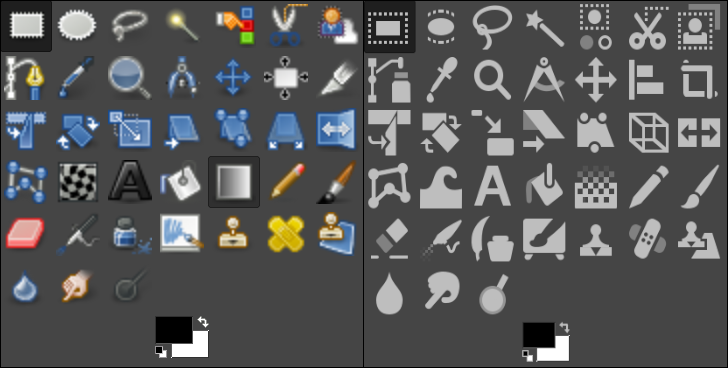
\includegraphics[width=0.50\textwidth]{Images/28to210_icons}
        \caption{Ancien et nouveau set d'icônes}
    \end{figure} 
	Pour plus d'infos sur ce qui a changé avec la mise à jour 2.10:
    \fbox{\url{https://www.gimp.org/release-notes/gimp-2.10.html}}
    \end{center}
\end{frame}

\section{Présentation de l'interface et des outils}
\begin{frame}[allowframebreaks]{L'interface}
    \begin{figure}
        \centering
        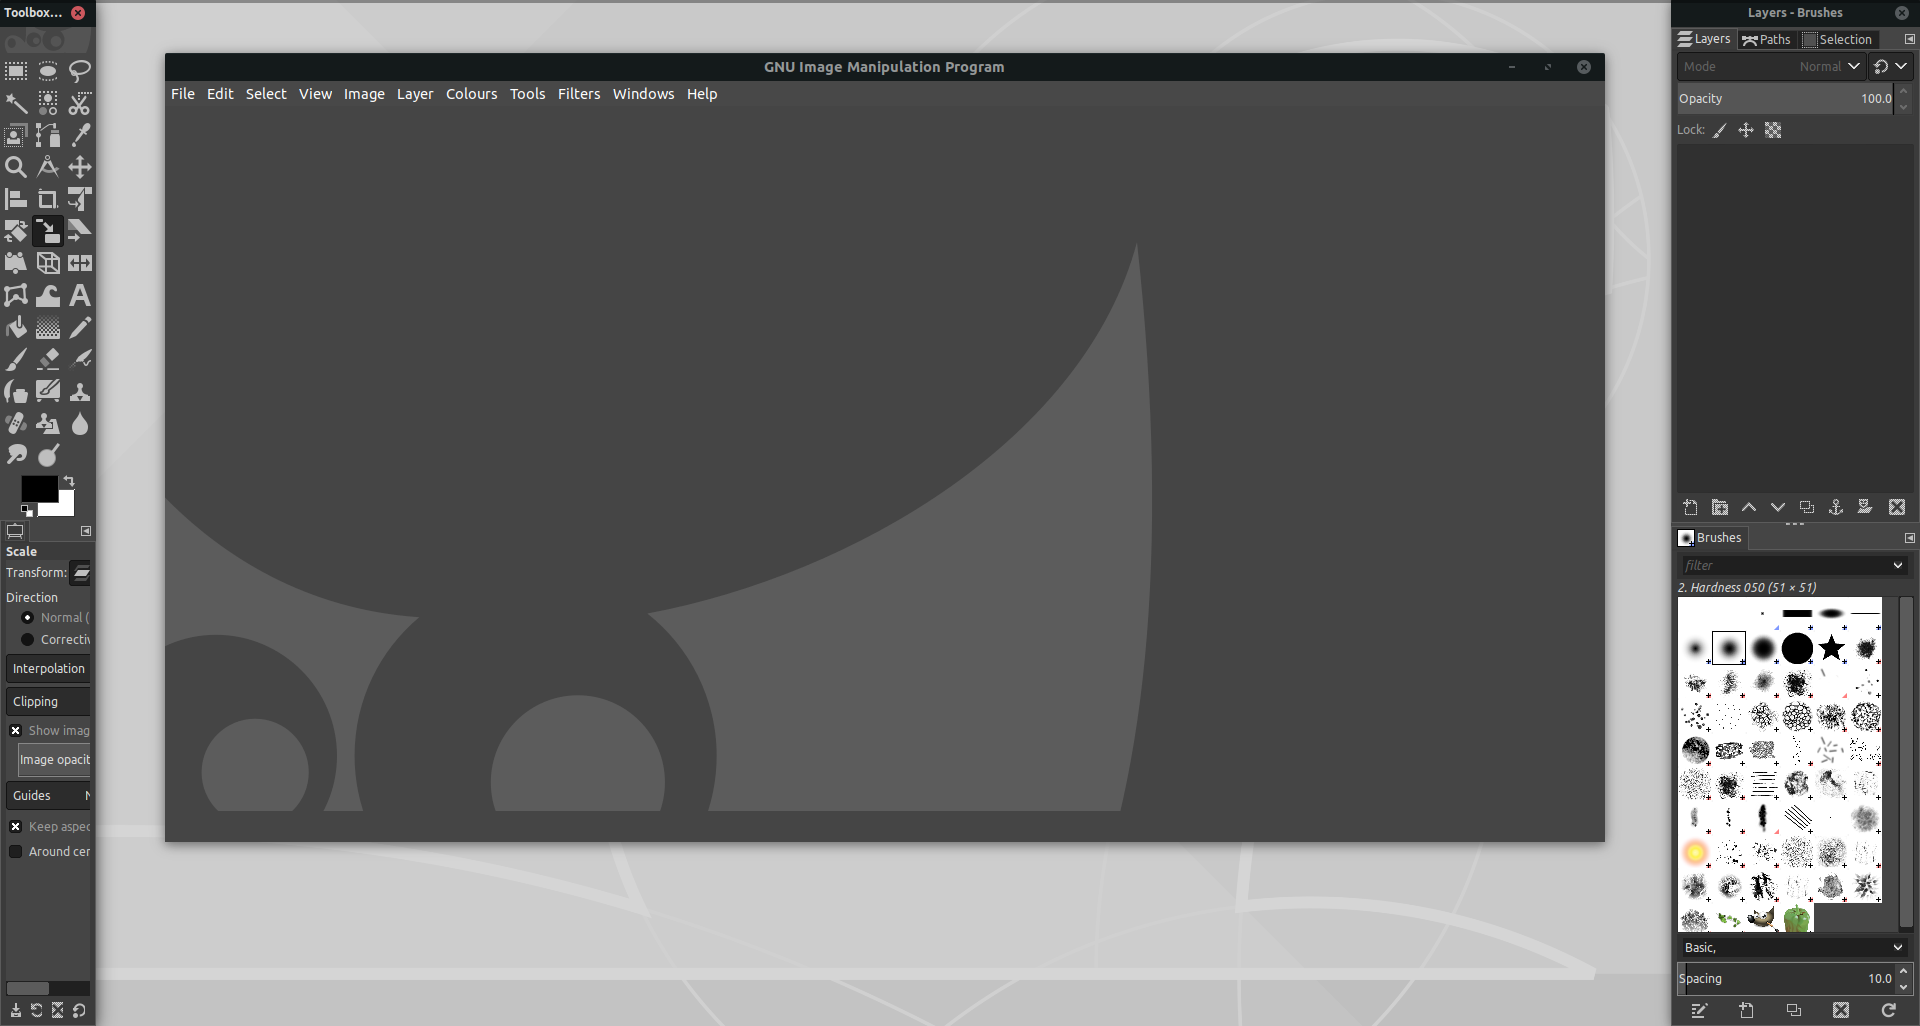
\includegraphics[width=0.9\textwidth]{Images/gimp_multiple_windows}
        \caption{L'interface multi-fenêtres}
    \end{figure} 
    \framebreak
    \begin{center}
        Fenêtres > Mode fenêtre unique
        \begin{figure}
            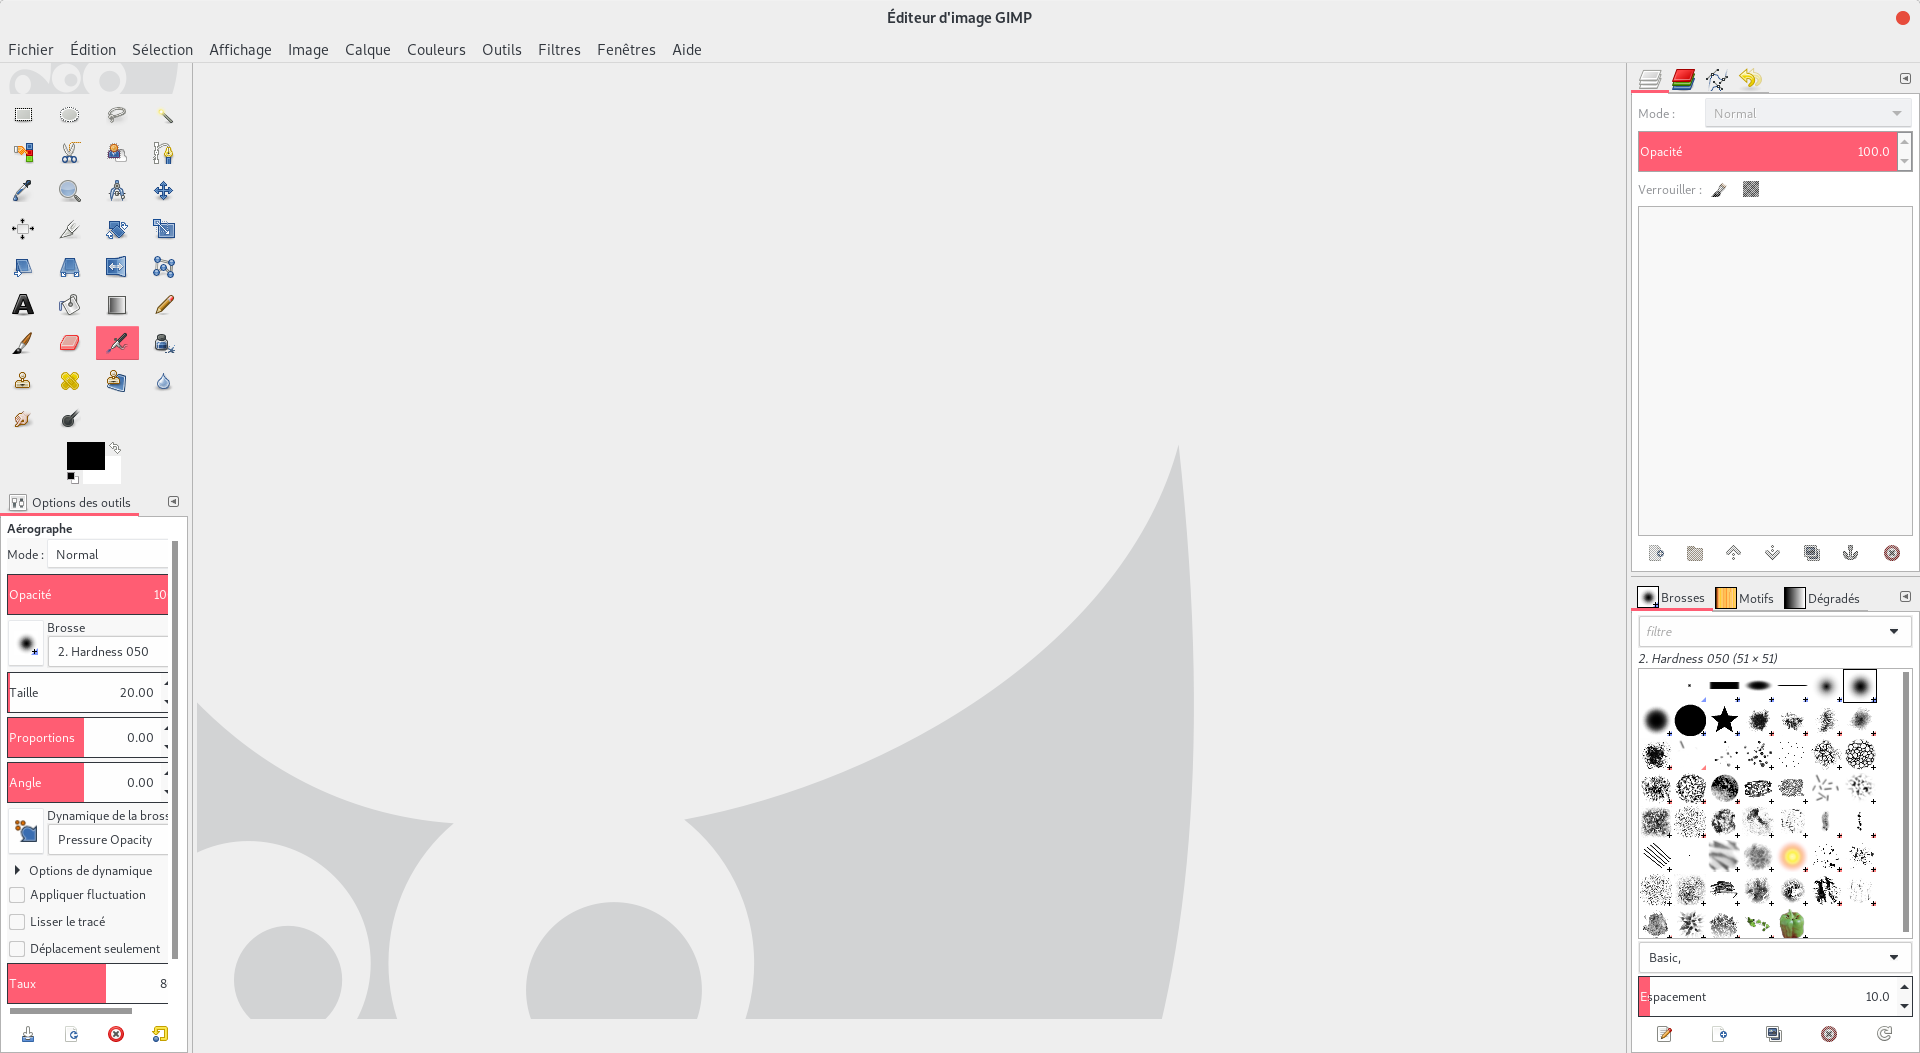
\includegraphics[width=0.9\textwidth]{Images/gimp_single_window}
            \caption{L'interface fenêtre unique}
        \end{figure}
    \end{center}
\end{frame}

\begin{frame}{Créer/importer une image}
	\begin{itemize}
		\item Pour \textbf{créer} une image: Fichier > Nouvelle image ou \keys{\ctrl + N}
			\begin{itemize}
				\item Sélectionnez un modèle (A3, A4, A5...) ou spécifier manuellement les dimensions (en pixels, mm, cm...).
			\end{itemize}
		\item Pour \textbf{importer} une image: Fichier  > Ouvrir ou \keys{\ctrl + O}.
			\begin{itemize}
				\item GIMP supporte de nombreux formats: PNG, JPEG, GIF...
			\end{itemize}
		\item Pour \textbf{créer} depuis le presse-papiers (copier/coller): Créer > Depuis le presse-papiers ou \keys{\shift + \ctrl + V}
	\end{itemize}
	\begin{center}
		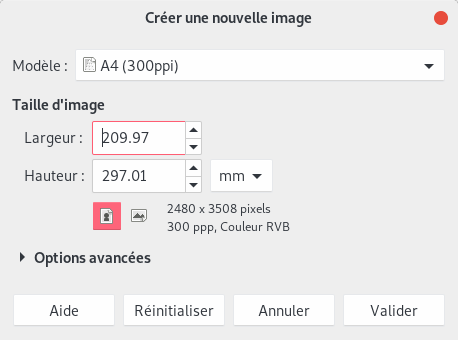
\includegraphics[width=0.5\textwidth]{Images/new_image.png}
	\end{center}
\end{frame}

\begin{frame}{Une image c'est quoi ?}
	\begin{center} 
		\textbf{Image matricielle} $\leftrightarrow$ Image vectorielle 
		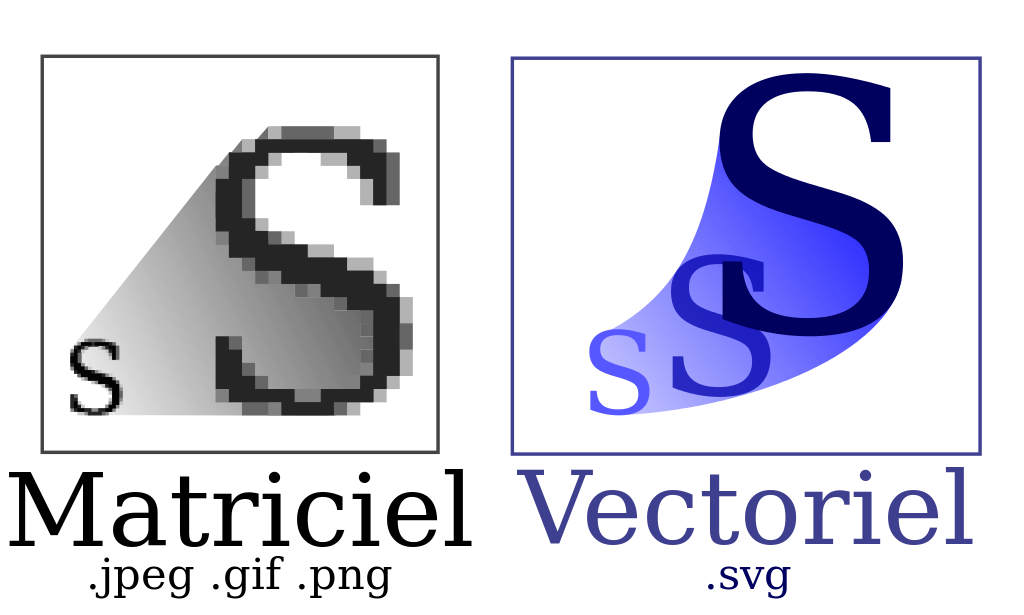
\includegraphics[width=0.6\textwidth]{Images/mat_vs_vec}
	\end{center}
	Pourquoi n'utilise-t-on pas toujours des images vectorielles ? 
	\begin{itemize}
		\item les images vectorielles ne peuvent afficher que des images construites à l'aide de formes. Les images matricielles ont l'avantage d'être définies au pixel près.
	\end{itemize}
\end{frame}

\begin{frame}{Les formats}
	Stocker chaque pixel demande beaucoup de mémoire. Solution ? Compresser les images:
	\begin{itemize}
		\item compression sans pertes (PNG, GIF);
		\item compression avec pertes (JPEG).
	\end{itemize}
	Les trois principaux formats d'images sont
	\begin{itemize}
		\item \textbf{JPEG}: léger (mais avec pertes), idéal pour les photos;
		\item \textbf{PNG}: plus lourd que JPEG (mais sans pertes), très bon support de la transparence;
		\item \textbf{GIF}: support des animations, limité à 256 couleurs.
	\end{itemize}
	Un projet GIMP sera sauvegardé au format \textbf{XCF}, un format d'image libre qui contiendra les différents calques et paramètres de votre création.
	
	L'équivalent d'Adobe Photoshop est le format \textbf{PSD}.
\end{frame}

\begin{frame}{Enregistrement et exportation}
	\begin{itemize}
		\item Pour \textbf{enregistrer} au format \textbf{XCF}: Fichier > Enregistrer ou \keys{\ctrl + S}.
		\item Pour \textbf{exporter} votre image dans un autre format: Fichier > Exporter ou \keys{\shift + \ctrl + E}.
	\end{itemize}
	\begin{center}
		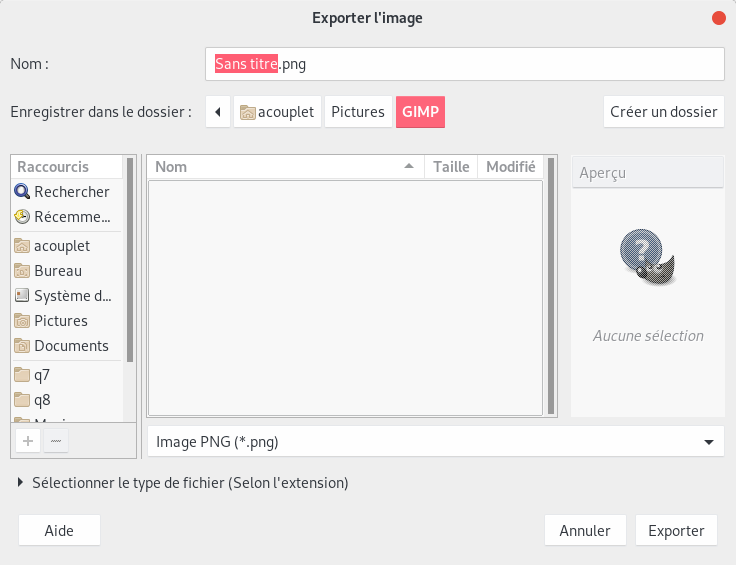
\includegraphics[width=0.5\textwidth]{Images/export}
	\end{center}
\end{frame}

\begin{comment}
\begin{frame}{Les couleurs}
	Il est possible de gérer 2 couleurs: les couleurs de premier et d'arrière-plan:
	\begin{center}
		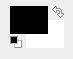
\includegraphics[width=0.08\textwidth]{Images/color_primary}
	\end{center}
	Il suffit de cliquer sur une de ces couleurs pour la modifier:
	\begin{center}
		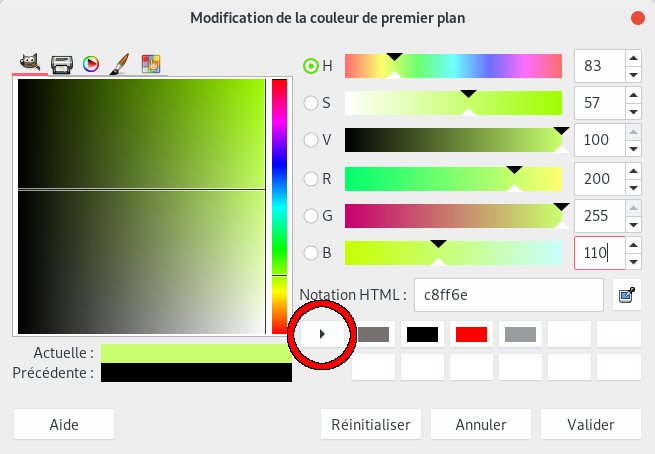
\includegraphics[width=0.5\textwidth]{Images/color_selector}
	\end{center}
	Il est possible de sélectionner une couleur ou de rentrer ses valeurs RGB. Une fois votre couleur choisie, vous pouvez l'ajouter à votre palette.
\end{frame}

\begin{frame}[allowframebreaks]{Les outils de coloration}
	La \textbf{pipette} permet de récupérer la couleur d'un pixel d'une image en cliquant sur le pixel en question.
	\begin{center}
		
\includegraphics[width=0.05\textwidth]{Images/color_tool_0}
		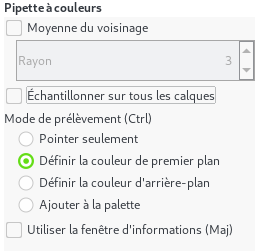
\includegraphics[width=0.3\textwidth]{Images/color_tool_0_settings}
	\end{center}
	L'outil permet de définir la couleur de premier plan, la couleur d'arrière-plan ou simplement d'ajouter la couleur à la palette.
	
	\framebreak
	Le \textbf{pot de peinture} permet de remplir une zone.
	\begin{center}
		
\includegraphics[width=0.05\textwidth]{Images/color_tool_1}
		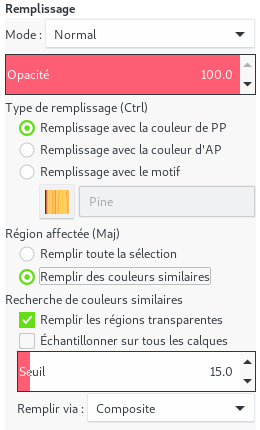
\includegraphics[width=0.25\textwidth]{Images/color_tool_1_settings}
	\end{center}
	Le seuil permet d'ajuster la zone à remplir: 
	\begin{center}
		
\includegraphics[width=0.3\textwidth]{Images/color_tool_1_test0}
		
\includegraphics[width=0.3\textwidth]{Images/color_tool_1_test1}
		
\includegraphics[width=0.3\textwidth]{Images/color_tool_1_test2}
	\end{center}
	\begin{scriptsize}
	Exemple: image originale, remplissage noir avec seuil à 30, remplissage noir avec seuil à 60.
	\end{scriptsize}
	
	\framebreak
	L'outil de gradient permet de créer des dégradés entre la couleur de premier plan et celle d'arrière-plan.
	\begin{center}
		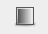
\includegraphics[width=0.05\textwidth]{Images/color_tool_2}
		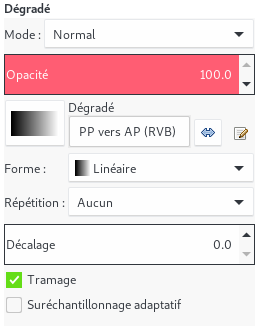
\includegraphics[width=0.3\textwidth]{Images/color_tool_2_settings}
	\end{center}
	Il existe de nombreux modes et de nombreuses formes, n'hésitez pas à les essayer pour les découvrir. 
	
\end{frame}
\end{comment}

\begin{frame}[allowframebreaks]{Les outils}
	
	\begin{figure}
        	\centering
        	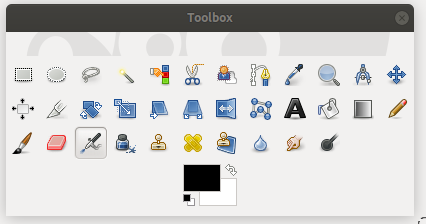
\includegraphics[width=0.4\textwidth]{Images/gimp_toolbox}
        	\caption{La boîte à outils de GIMP} 
    	\end{figure}
	
	\textbf{Accès}
	
	\begin{itemize}
		\item Fenêtres > Boîte à outils
		\item Outils > Boîte à outils
	\end{itemize}
	
	\vspace{0.2cm}
	\textbf{Raccourci} \keys{\ctrl + B}
	
	\framebreak
	\textbf{Paramètres} \textit{double} cliquer sur l'icône de l'outil concerné
	\begin{figure}
        	\centering
        	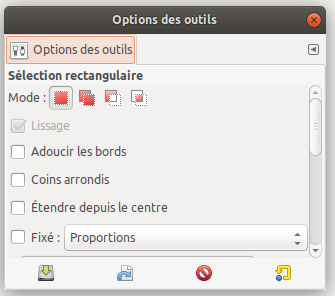
\includegraphics[width=0.4\textwidth]{Images/option_outil}
        	\caption{Exemple : paramètres de l'outil de sélection} 
    	\end{figure}

\end{frame}	

\begin{frame}[allowframebreaks]{Les outils de sélection}
\begin{enumerate}

	
	\tool{Rectangulaire}{R}{rectangle.png}
	
	\vspace{0.5cm}
	\begin{minipage}[t]{0.45\textwidth}
	Options (\textit{fixé}) : 
		
	\begin{itemize}
		\item Position
		\item Proportions fixées
		\item Hauteur fixée
		\item Largeur fixée
	\end{itemize}
	\end{minipage}
	\begin{minipage}[t]{0.45\textwidth}
	
	\begin{figure}
        	\centering
        	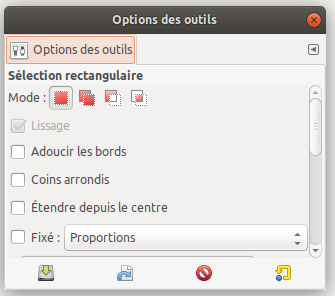
\includegraphics[width=\textwidth]{Images/option_outil} 
	\end{figure}
	\end{minipage}
	
	\framebreak
	
	
	\tool{Elliptique}{E}{ellipse.png}	
	
	\vspace{0.5cm}
	\begin{minipage}[t]{0.45\textwidth}
	Options (\textit{fixé}) : 
		
	\begin{itemize}
		\item Position
		\item Proportions fixées
		\item Hauteur fixée
		\item Largeur fixée
	\end{itemize}
	\end{minipage}
	\begin{minipage}[t]{0.45\textwidth}
	
	\begin{figure}
        	\centering
        	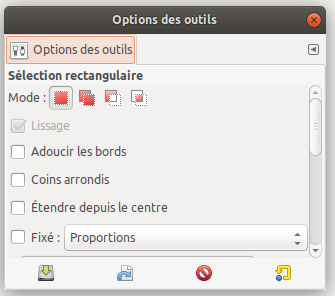
\includegraphics[width=\textwidth]{Images/option_outil} 
	\end{figure}
	\end{minipage}
	
	\framebreak 
	
	
	
	
	\tool{Ciseaux intelligents}{I}{smart_cut.png}
	
	\begin{minipage}{0.45\textwidth}
	\begin{figure}
        	\centering
        	
\includegraphics[width=\textwidth]{Images/gimp-logo.png} 
	\end{figure}
	\end{minipage}\hfill
	\begin{minipage}{0.45\textwidth}
	\begin{figure}
        	\centering
        	
\includegraphics[width=\textwidth]{Images/smart_ex.png} 
	\end{figure}
	\end{minipage}
	
	\vspace{0.4cm}
	\textbf{Attention} Une fois le contour terminé, cliquer au \textbf{centre} de celui-ci pour le valider
	
	\framebreak
	
	\tool{À main levée}{F}{freeSelect.png}

	\begin{itemize}
		\item \textbf{Trait continu} Maintenir le clic gauche 
	\end{itemize}
	
		\begin{minipage}{0.45\textwidth}
		\begin{figure}
        		\centering
        		
\includegraphics[width=\textwidth]{Images/gimp-logo.png} 
		\end{figure}
		\end{minipage}\hfill
		\begin{minipage}{0.45\textwidth}
		\begin{figure}
        		\centering
        		
\includegraphics[width=\textwidth]{Images/main_levee.png} 
		\end{figure}
		\end{minipage}
		
	\framebreak
	
	\setcounter{enumi}{3}
	\tool{À main levée}{F}{freeSelect.png}

	\begin{itemize}
		\item \textbf{Point par point} Clic pour chaque point successif 
	\end{itemize}
	
		\begin{minipage}{0.45\textwidth}
		\begin{figure}
        		\centering
        		
\includegraphics[width=\textwidth]{Images/gimp-logo.png} 
		\end{figure}
		\end{minipage}\hfill
		\begin{minipage}{0.45\textwidth}
		\begin{figure}
        		\centering
        		
\includegraphics[width=\textwidth]{Images/point_point.png} 
		\end{figure}
		\end{minipage}
	
		
		\framebreak		
		\tool{Par couleur}{Maj + 0}{colorSelect}
		
		\vspace{0.3cm}
		\begin{minipage}[t]{0.55\textwidth}
		Options : 
		
		\begin{itemize}
			\item Mode de sélection
			\item Seuil
			\item Echantillonner sur tous les calques
		\end{itemize}
		\end{minipage}
		\begin{minipage}[t]{0.35\textwidth}
		
		\begin{figure}
        		\centering
        		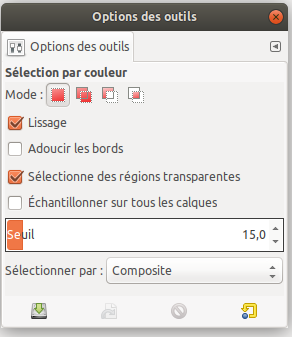
\includegraphics[width=\textwidth]{Images/opt_color_select} 
		\end{figure}
		\end{minipage}
		
		\framebreak
		
		\setcounter{enumi}{4}
		\tool{Par couleur}{Maj + 0}{colorSelect}
		
		\begin{minipage}{0.45\textwidth}

		\begin{figure}
        		\centering
        		
\includegraphics[width=\textwidth]{Images/gimp-logo.png} 
        		\caption{Figure originelle}
		\end{figure}
		\end{minipage}\hfill
		\begin{minipage}{0.45\textwidth}
		\begin{figure}
        		\centering
        		
\includegraphics[width=\textwidth, trim = 0 0.22cm 0 0, clip]{Images/color_ex.png} 
        		\caption{Zone sélectionnée (en \textbf{rouge})}
		\end{figure}
		\end{minipage}

\end{enumerate}
\end{frame}

\begin{frame}{Les outils de sélection}
\textbf{Paramètres de sélection}
\begin{figure}
        \centering
        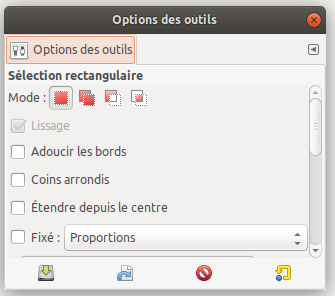
\includegraphics[width=0.4\textwidth]{Images/option_outil} 
\end{figure}

\begin{enumerate}
	\item \textbf{Remplacer} la sélection actuelle
	\item \textbf{Ajouter} à la sélection actuelle
	\item \textbf{Soustraire} à la sélection actuelle
	\item \textbf{Intersection} avec la sélection actuelle	
\end{enumerate}
\end{frame}

\begin{frame}{Les outils de sélection}
\textbf{Paramètres de sélection}
\begin{overprint}
\begin{figure}
        \centering
        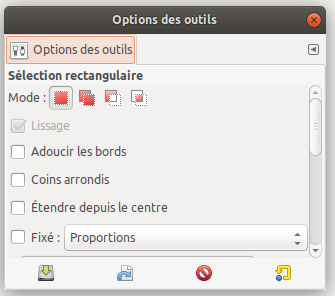
\includegraphics[width=0.4\textwidth, trim = 0 6.3cm 0 0, clip]{Images/option_outil} 
\end{figure}

\begin{enumerate}

	\only<1>{
	\item \textbf{Exemple}
	\begin{figure}
        	\centering
        	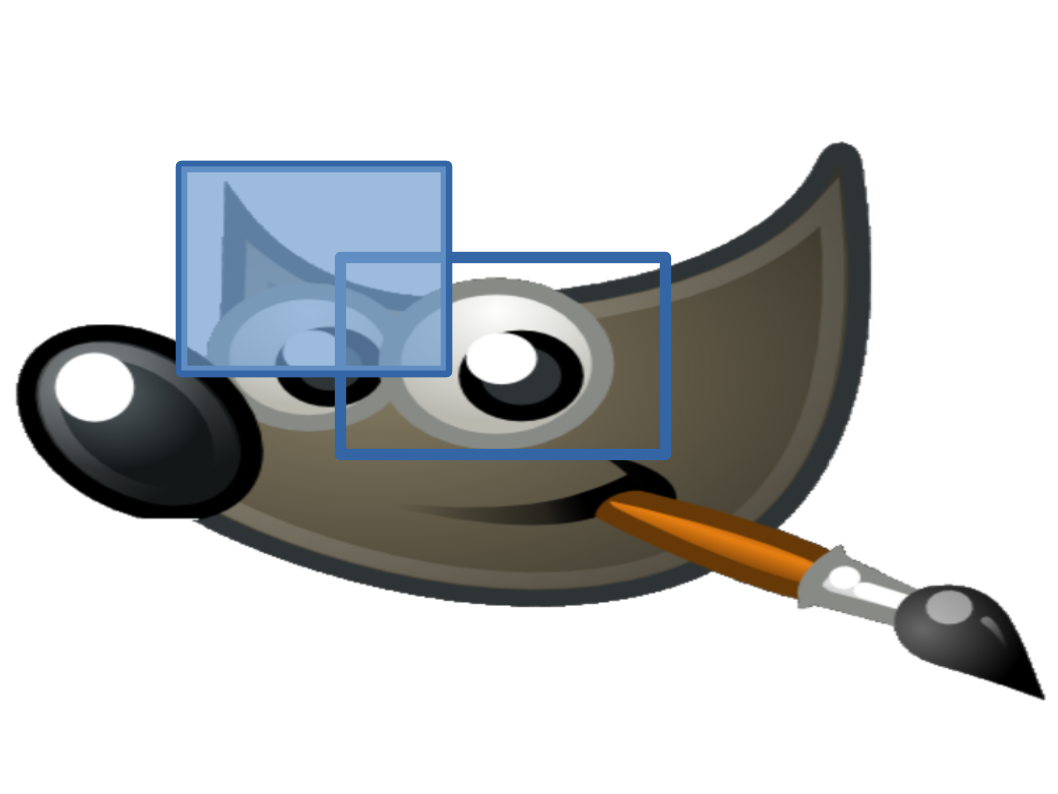
\includegraphics[width=0.4\textwidth]{Images/Selec1.png} 
	\end{figure}}
	
	\only<2>{
	\item[1] \textbf{Remplacer} la sélection actuelle
	\begin{figure}
        	\centering
        	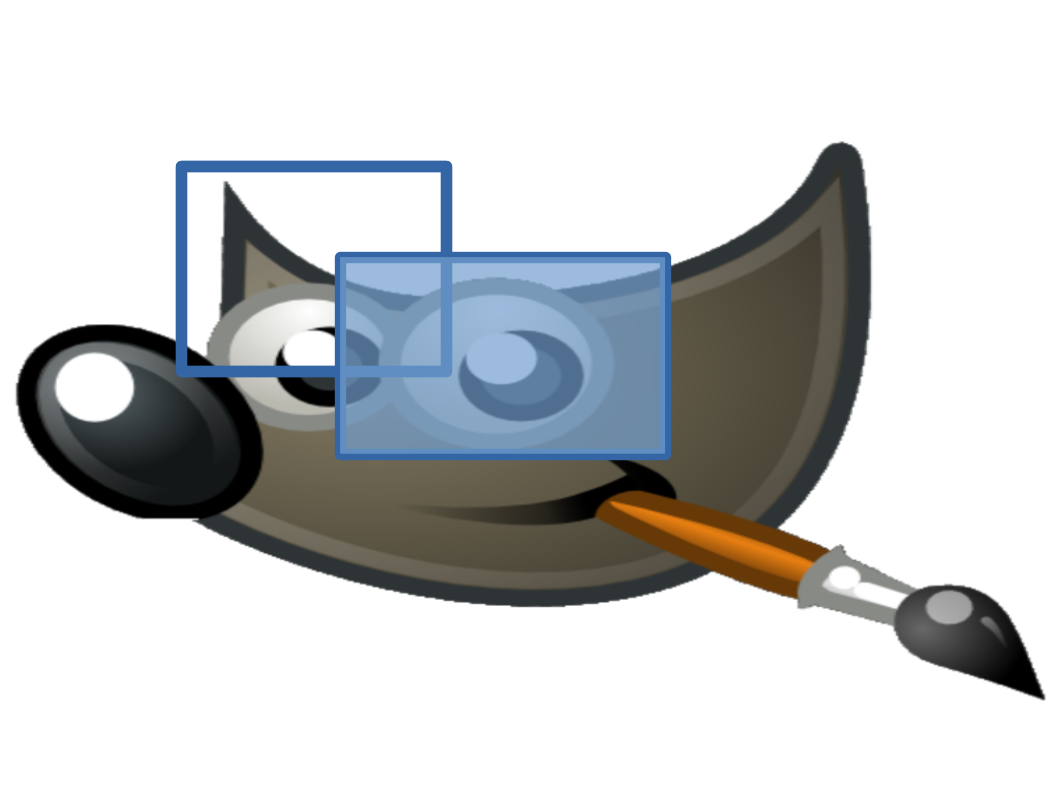
\includegraphics[width=0.4\textwidth]{Images/Selec5.png} 
	\end{figure}}
	
	\only<3>{	
	\item[2] \textbf{Ajouter} à la sélection actuelle
	\begin{figure}
        	\centering
        	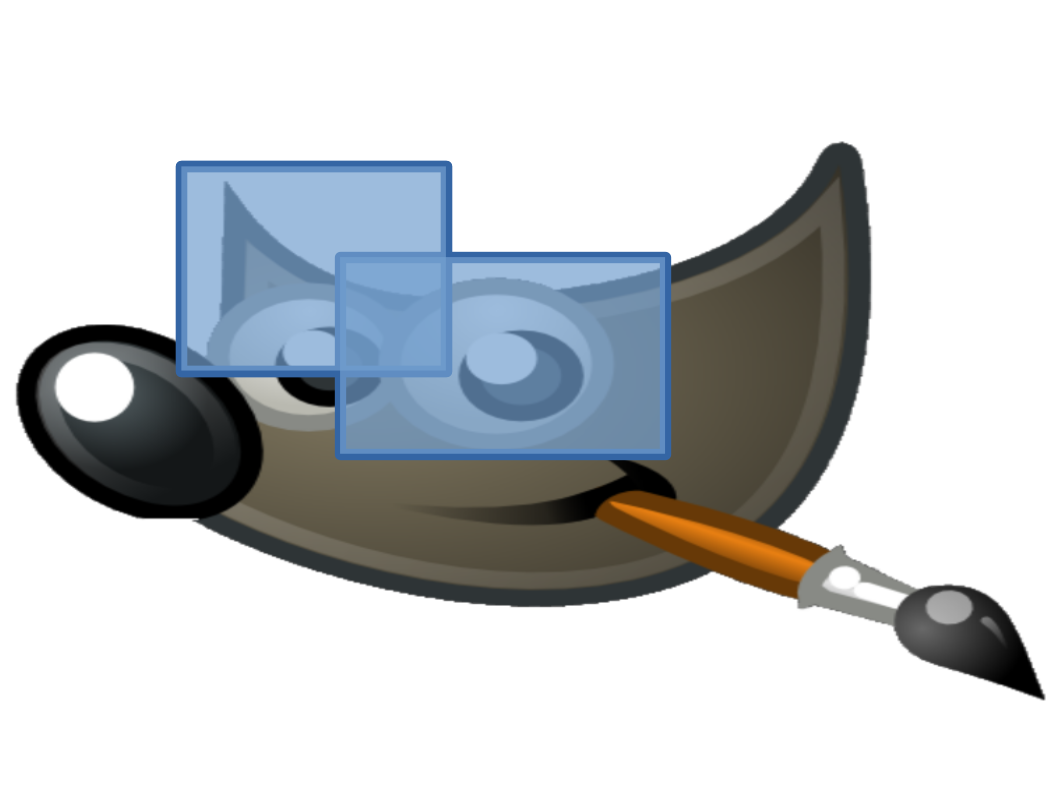
\includegraphics[width=0.4\textwidth]{Images/Selec2.png} 
	\end{figure}}
	
	\only<4>{
	\item[3] \textbf{Soustraire} à la sélection actuelle
	\begin{figure}
        	\centering
        	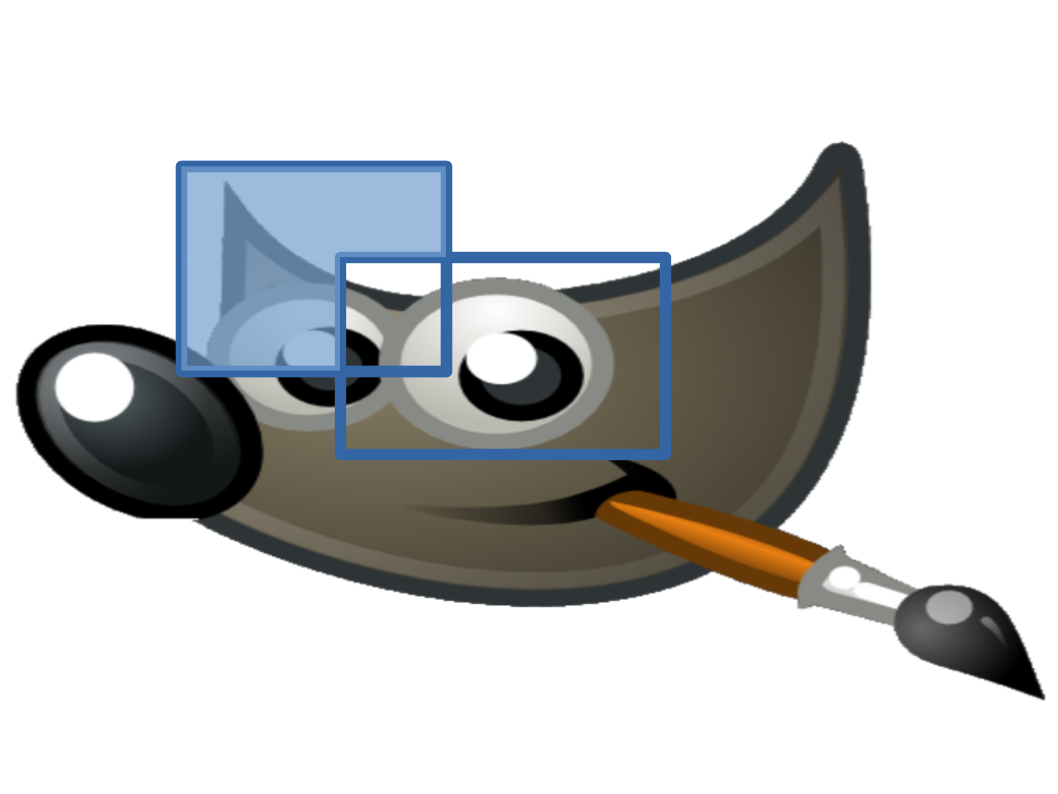
\includegraphics[width=0.4\textwidth]{Images/Selec3.png} 
	\end{figure}}
	
	\only<5>{
	\item[4] \textbf{Intersection} avec la sélection actuelle
	\begin{figure}
        	\centering
        	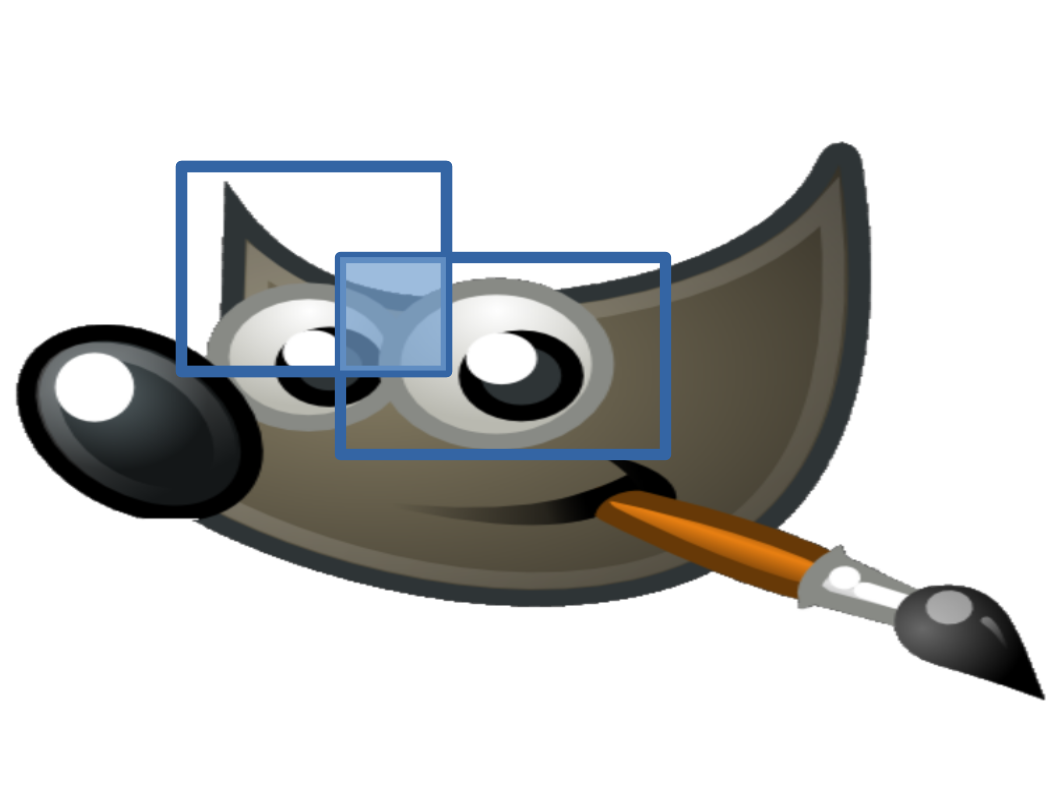
\includegraphics[width=0.4\textwidth]{Images/Selec4.png} 
	\end{figure}}
	
\end{enumerate}
\end{overprint}
\end{frame}

\begin{frame}[allowframebreaks]{Les outils de transformation}
\begin{enumerate}

	\tool{Rotation}{Maj+R}{rotate.png}
	\vspace{0.5cm}
	
	\begin{minipage}{0.45\textwidth}
	\begin{figure}
        	\centering
        	
\includegraphics[width=\textwidth]{Images/gimp-logo.png} 
	\end{figure}
	\end{minipage}\hfill
	\begin{minipage}{0.45\textwidth}
	\begin{figure}
        	\centering
        	
\includegraphics[width=0.8\textwidth]{Images/Rotate.png} 
	\end{figure}
	\end{minipage}
	\framebreak
	
	\tool{Agrandissement/Réduction}{Maj+T}{rescale.png}
	
	\begin{minipage}{0.45\textwidth}
	\begin{figure}
        	\centering
        	
\includegraphics[width=\textwidth]{Images/gimp-logo.png} 
	\end{figure}
	\end{minipage}\hfill
	\begin{minipage}{0.45\textwidth}
	\begin{figure}
        	\centering
        	
\includegraphics[width=\textwidth]{Images/redimension.png} 
	\end{figure}
	\end{minipage}
	\framebreak
	
	\tool{Inversion}{Maj+F}{flip.png}
	
	\begin{minipage}{0.45\textwidth}
	\begin{figure}
        	\centering
        	
\includegraphics[width=\textwidth]{Images/gimp-logo.png} 
	\end{figure}
	\end{minipage}\hfill
	\begin{minipage}{0.45\textwidth}
	\begin{figure}
        	\centering
        	
\includegraphics[width=\textwidth]{Images/Flip.png} 
	\end{figure}
	\end{minipage}
	
	\framebreak
	\setcounter{enumi}{2}	
	\tool{Inversion}{Maj+F}{flip.png}
	
	\begin{minipage}{0.45\textwidth}
	\begin{figure}
        	\centering
        	
\includegraphics[width=\textwidth]{Images/gimp-logo.png} 
	\end{figure}
	\end{minipage}\hfill
	\begin{minipage}{0.45\textwidth}
	\begin{figure}
        	\centering
        	
\includegraphics[width=\textwidth]{Images/Flip2.png} 
	\end{figure}
	\end{minipage}
	\framebreak
	
	\tool{Cisaillement}{Maj+S}{shear.png}
	\vspace{0.5cm}
	
	\begin{minipage}{0.45\textwidth}
	\begin{figure}
        	\centering
        	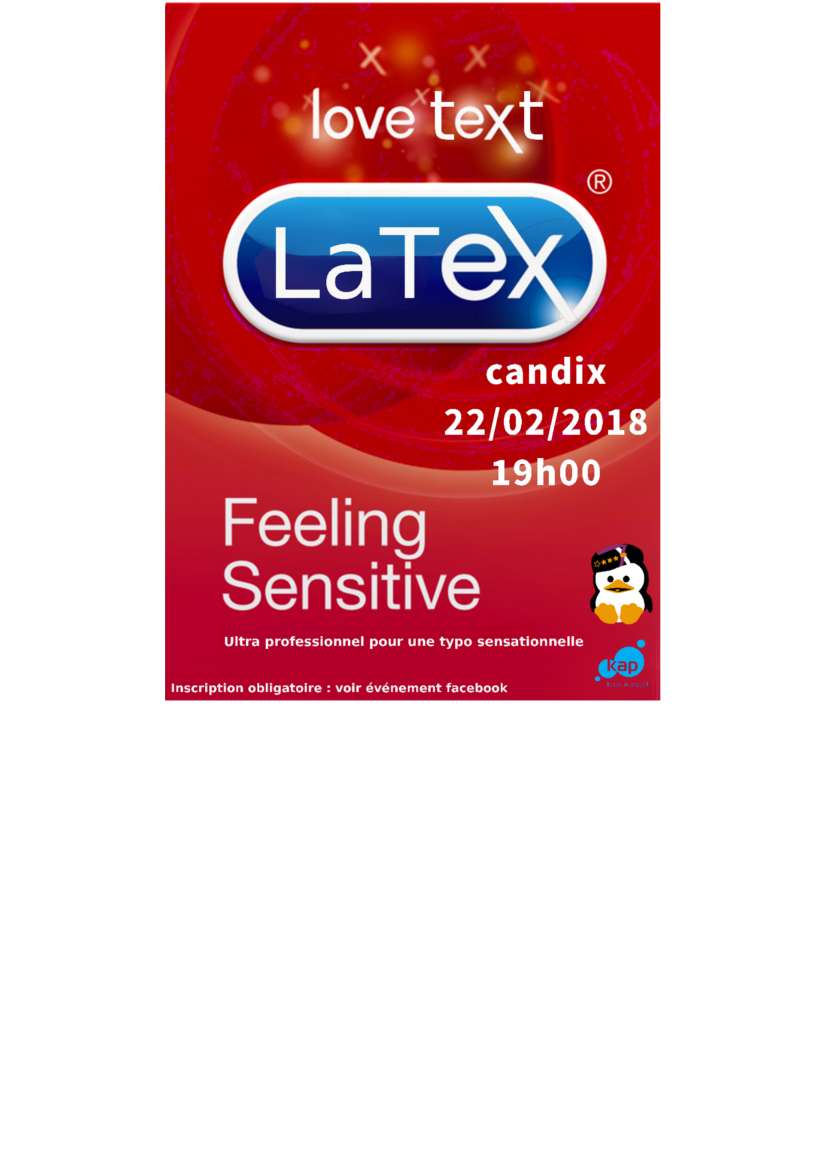
\includegraphics[width=0.8\textwidth]{Images/NoShear.png} 
	\end{figure}
	\end{minipage}\hfill
	\begin{minipage}{0.45\textwidth}
	\begin{figure}
        	\centering
        	\includegraphics[width=0.8\textwidth]{Images/Shear.png} 
	\end{figure}
	\end{minipage}
	\framebreak
	
	\tool{Mise en perspective}{Maj+R}{perspective.png}
	\vspace{0.3cm}
	
	\begin{minipage}{0.45\textwidth}
	\begin{figure}
        	\centering
        	\includegraphics[width=0.5\textwidth]{Images/FullTex.png} 
	\end{figure}
	\end{minipage}\hfill
	\begin{minipage}{0.45\textwidth}
	\begin{figure}
        	\centering
        	\includegraphics[width=0.5\textwidth]{Images/Perspective.png} 
	\end{figure}
	\end{minipage}
	\framebreak
	
	\tool{Découpe}{Maj+C}{cutTool.png}
	
	\begin{minipage}{0.45\textwidth}
	\begin{figure}
        	\centering
        	\includegraphics[width=\textwidth]{Images/gimp-logo.png} 
	\end{figure}
	\end{minipage}\hfill
	\begin{minipage}{0.45\textwidth}
	\begin{figure}
        	\centering
        	\includegraphics[width=0.6\textwidth]{Images/cut.png} 
	\end{figure}
	\end{minipage}
\end{enumerate}
\end{frame}


\begin{frame}{Les outils de coloration}

\textbf{Couleurs actives}


%\begin{overprint}
%\begin{figure}
%	\centering
%	\begin{tikzpicture}[scale=0.7, transform shape]
%        \node[anchor=south west,inner sep=0] at (0.4,0) {\includegraphics[width=0.1\textwidth]{Images/gimp_couleurs_actives}};
%        \onslide<2>{\draw[teal,ultra thick,rounded corners] (0.25,0.3) rectangle (1.5,1); 
%        \node [anchor=center, teal] (note) at (0.7,1.4) {\Large Avant-plan \textcolor{black}{{\small (Clic \textbf{gauche})}}};}
%	\onslide<3>{\draw[red,ultra thick,rounded corners] (0.6,0) rectangle (1.55,0.7);
%        \node [anchor=center, red] (Inner) at (0.7,-0.3) {\Large Arrière-plan \textcolor{black}{{\small (Clic \textbf{droit})}}};}
%    	\end{tikzpicture} 
%	\includegraphics[width=0.1\textwidth]{Images/gimp_couleurs_actives}
%\end{figure}

%\vspace{-0.6cm}
%\textbf{Palette des couleurs} Double clique sur l'une des couleurs actives


%\begin{figure}
%	\centering
%	\begin{tikzpicture}[scale=1, transform shape]
%        \node[anchor=south west,inner sep=0] at (0.4,0) {\includegraphics[width=0.4\textwidth]{Images/gimp_color_box}};

%        \onslide<4>{\draw[red,ultra thick,rounded corners] (4.2,1.2) rectangle (4.6,1.6); 
%        \node [anchor=center, red] (note) at (3.7,-0.3) {\Large Sélection \\de couleur};}
%    \end{tikzpicture} 
%	\includegraphics[width=0.1\textwidth]{Images/gimp_couleurs_actives}
%\end{figure}


%\end{overprint}


%\begin{overprint}
\begin{figure}
	\centering
	\begin{tikzpicture}[scale=0.7, transform shape]
        \node[anchor=south west,inner sep=0] at (0.4,0) {\includegraphics[width=0.1\textwidth]{Images/gimp_couleurs_actives}};
        \onslide<2>{\draw[teal,ultra thick,rounded corners] (0.25,0.3) rectangle (1.5,1); 
        \node [anchor=center, teal] (note) at (0.7,1.4) {\Large Avant-plan \textcolor{black}{{\small (Clic \textbf{gauche})}}};}
	\onslide<3>{\draw[red,ultra thick,rounded corners] (0.6,0) rectangle (1.55,0.7);
        \node [anchor=center, red] (Inner) at (0.7,-0.3) {\Large Arrière-plan \textcolor{black}{{\small (Clic \textbf{droit})}}};}
    	\end{tikzpicture} 
\end{figure}

\vspace{-0.2cm}
\textbf{Palette des couleurs} Double clique sur l'une des couleurs actives


\begin{figure}
	\centering
	\begin{tikzpicture}[scale=1, transform shape]
        \node[anchor=south west,inner sep=0] at (0.4,0) {\includegraphics[width=0.4\textwidth]{Images/gimp_color_box}};

        \onslide<4>{\draw[red,ultra thick,rounded corners] (4.2,1.2) rectangle (4.6,1.6); 
        \node [anchor=center, red] (note) at (3.7,-0.4) {\Large Sélection de couleur};}
    	\end{tikzpicture} 
\end{figure}
%\end{overprint}



\end{frame}


\begin{frame}{Les outils de coloration}
\begin{minipage}[t]{0.49\textwidth}
	\textbf{Code HTML}
	
	\vspace{0.2cm}
	Couleurs pré-définies
	
	\vspace{0.2cm}
	
	\begin{center}
	\fbox{\parbox{0.7\linewidth}{%
	\url{https://www.toutes-les-couleurs.com/code-couleur-html.php}	
	}}
	\end{center}

\end{minipage}\hfill
\begin{minipage}[t]{0.49\textwidth}
	\textbf{Code RGB}
	
	\begin{itemize}
		\item[H] Teinte
		\item[S] Valeur 
		\item[V] Saturation
		\item[R] Rouge
		\item[G] Vert 
		\item[B] Bleu
	\end{itemize}
	
\end{minipage}

\end{frame}


\begin{frame}[allowframebreaks]{Les outils de coloration}
	
	\begin{itemize}
	\tool{Sélection de couleur}{O}{colorProbe.png}
	
	\vspace{0.5cm}
	\tool{Outil de remplissage}{Maj + B}{bucketFill.png}
	
	\tool{Crayon}{N}{pen.png}
	
	\tool{Pinceau}{P}{paintbrush.png}
	
	\tool{Aérograhe}{A}{aero.png}
	

	
	\framebreak
	\tool{Dégradé}{L}{colorTool2.png}
	
	\begin{minipage}{0.45\textwidth}
	\begin{figure}
        	\centering
        	\includegraphics[width=\textwidth]{Images/degrade_ex.png} 
	\end{figure}
	\end{minipage}\hfill
	\begin{minipage}{0.45\textwidth}
	\begin{figure}
        	\centering
        	\includegraphics[width=\textwidth]{Images/degrade_ex2.png} 
	\end{figure}
	\end{minipage}
	
	
	Tracer des \textbf{lignes droites} : \textbf{majuscule enfoncée} entre deux points sélectionnés
	\end{itemize}
\end{frame}

%\begin{frame}{L'outil de texte}

%\end{frame}

\begin{frame}[allowframebreaks]{Autres outils}
\begin{enumerate}
	\tool{Zoom}{Z}{zoom.png}
	
	\textbf{Raccourci} \keys{{+}}, \keys{-}, \keys{1}, \keys{2}, \keys{3}, \keys{4} et \keys{5}
	\vspace{0.6cm}
	
	\tool{Déplacement}{M}{moove.png}
	
	\framebreak
	\tool{Alignement}{Q}{autopose.png}
	
	\begin{figure}
        	\centering
        	\includegraphics[width=0.3\textwidth]{Images/automoove_opt.png} 
	\end{figure}
	
\end{enumerate}
\end{frame}

\begin{frame}[allowframebreaks]{Les mesures}
\begin{itemize}
	\item \textbf{Echelle graduée} aux \textit{extrémités} de l'image
	
	\begin{figure}
        	\centering
        	\includegraphics[width=0.3\textwidth]{Images/Scale.png} 
        \end{figure}

	\vspace{0.3cm}	
	
	\item Zone de \textbf{"Communication"} dans le \textit{coin inférieur droit}

	\begin{figure}
        	\centering
        	\includegraphics[width=0.3\textwidth]{Images/commu.png} 
	\end{figure}
	
	\framebreak
	\tool{Outil de mesure}{Maj + M}{measure.png}
	\begin{minipage}{0.45\textwidth}
	\begin{figure}
        	\centering
        	\includegraphics[width=\textwidth]{Images/gimp-logo.png} 
	\end{figure}
	\end{minipage}\hfill
	\begin{minipage}{0.45\textwidth}
	\begin{figure}
        	\centering
        	\includegraphics[width=\textwidth]{Images/measure_gimp.png} 
	\end{figure}
	\end{minipage}
	
	\begin{itemize}
		\item \textbf{Maintenir} le clic gauche entre les deux zones de mesure
		\item \textbf{Résultats} dans la zone \textit{inférieure droite} de l'écran
	\end{itemize}
\end{itemize}
\end{frame}

\begin{frame}[allowframebreaks]{Les calques}
	\begin{figure}
        	\centering
        	\includegraphics[width=0.3\textwidth]{Images/gimp_calques}
        	%\caption{Fenêtre de calques de GIMP} 
    	\end{figure}
    	
	\textbf{Accès} Fenêtres > Calques
	
	\vspace{0.2cm}
	\textbf{Raccourci} \keys{\ctrl + L}
	
	\framebreak
	
	\begin{figure}
        	\centering
        	\includegraphics[width=0.5\textwidth]{Images/Calque.jpg}
    	\end{figure}
	
	\begin{itemize}
		\item \textbf{Superposition} d'images
		\begin{itemize}
			\item \textit{Avant-plan} : le plus haut
			\item \textit{Arrière-plan} : le plus bas
		\end{itemize}
		\item Visible ou non 
		\item Ancrable
		\item Indépendant
	\end{itemize}	
	
	%\begin{enumerate}
	%	\item Chaque calque s'utilises \textbf{Indépendemment}
	%\end{enumerate}

\end{frame}


\begin{frame}[allowframebreaks]{Exercice I}
	Image de départ: \href{http://louvainlinux.github.io/atelier-gimp/src/Images/ex1/original.jpg}{Lien de l'image}
	\begin{center}
	\includegraphics[width=0.45\textwidth]{Images/ex1/Ex1_step0.jpg}
	\includegraphics[width=0.45\textwidth]{Images/ex1/Ex1_step5.jpg}
	\end{center}
	\framebreak
	Découpe de l'image
	\begin{center}
		\includegraphics[width=0.4\textwidth]{Images/ex1/Ex1_step1.jpg}
	\end{center}
	\framebreak
	Inversion de l'image
	\begin{center}
		\includegraphics[width=0.4\textwidth]{Images/ex1/Ex1_step2.jpg}
	\end{center}
	\framebreak
	Coloration de zones du ballon en R=237, G=178 et B=35.
	\begin{center}
		\includegraphics[width=0.4\textwidth]{Images/ex1/Ex1_step3.jpg}
	\end{center}
	\framebreak
	Mise en place d'un cadre
	\begin{center}
		\includegraphics[width=0.4\textwidth]{Images/ex1/Ex1_step4.jpg}
	\end{center}
	\framebreak
	Texte en rouge
	\begin{center}
		\includegraphics[width=0.4\textwidth]{Images/ex1/Ex1_step5.jpg}
	\end{center}
\end{frame}



\section{La modification non-destructrice}
	\begin{frame}{La modification non-destructrice}
	\framesubtitle{A quoi ça sert?}
	\begin{itemize}
		\item On peut revenir en arrière après avoir enregistré et rouvert son fichier
		\item Plus de possibilité de réparer ses erreurs
		\item Plus de possibilité de ne pas avoir à recommencer depuis le début...
		\item On évite les pertes d'information liées à la compression (jpeg par exemple)
	\end{itemize}		
	\end{frame}

	\begin{frame}{La modification non-destructrice}
	\framesubtitle{Comment ça fonctionne?}
	Le logiciel ne va plus directement altérer les pixels, mais enregistrer les modifications dans des fichiers annexes ou dans le document même (le format .xcf, pour gimp).
	\begin{itemize}
	\item On va utiliser au maximum les calques, quitte à en abuser
	\item Lâcher la gomme au profit des masques
	\item Appliquer localement les modifications avec les deux premiers points
	\end{itemize}		
	\end{frame}



%%% MASQUES de FUSION%%
\section{Masques de Fusion}
	\begin{frame}{Masques de Fusion}
		Les masques de fusion permettent de cacher une certaine partie d'un calque.
		$\Rightarrow$ Clic droit sur le calque $\rightarrow$ Add Layer Mask ...
		
		Conseil: sélectionner d'abord la zone à masquer
		\begin{center}
			\begin{figure}		
				\includegraphics[scale=.15]{Images/mask/mask1} 				
			\end{figure}	
		\end{center}
	\end{frame}

	\begin{frame}{Masques de Fusion}
		Il suffit maintenant de dessiner en noir ou blanc sur le masque de fusion pour faire apparaître (ou disparaiître) certaines zones du calque!
		\begin{itemize}
			\item Blanc $\Longrightarrow $ opaque
			\item Noir $ \Longrightarrow $ transparent
		\end{itemize}
		\begin{center}
			\begin{figure}
				\includegraphics[scale=.15]{Images/mask/mask3}		
			\end{figure}
		\end{center}
	\end{frame}
	
	\begin{frame}{Masques de Fusion}
		"Mais ça a l'air super compliqué! Pourquoi j'utiliserais ça et pas ma gomme?"
		
		Et bien, pour transformer ceci...
		
		\begin{figure}[H]
			\centering
			\begin{minipage}{.5\textwidth}
				\centering
				\includegraphics[height=100px]{Images/purge/Apollo_15_flag,_rover,_LM,_Irwin}
			\end{minipage}%
			\begin{minipage}{.5\textwidth}
				\centering
				\includegraphics[height=100px]{Images/mask/Conference_Solvay_Original}
			\end{minipage}
		\end{figure}
				
		
	\end{frame}		
	
	\begin{frame}{Masques de Fusion}
		... En ceci, sans trop se casser la tête car la gomme est "destructive".
	
		\begin{figure}[H]
			\centering
			\includegraphics[height=150px]{Images/mask/Conference_Solvay}
			\caption{\scriptsize{1927 Solvay Conference on Quantum Mechanics.}}
		\end{figure}
	
	\end{frame}		



	\begin{frame}{Masques de Fusion}
	\begin{overprint}
	\begin{enumerate}	
	\only<1>{		
		\framesubtitle{Intégrer un élément dans un image}
		
		\item[1.] \textbf{Sélectionner} la partie à intégrer et la masquer
		\begin{figure}
		\centering
			\begin{minipage}{.6\textwidth}
				\centering
				\includegraphics[height=125px]{Images/mask/mask4}
			\end{minipage}%
			\begin{minipage}{.4\textwidth}
				\centering
				\includegraphics[height=100px]{Images/mask/mask4_2}
			\end{minipage}	
		\end{figure}}
		
	\only<2>{		
		\framesubtitle{Intégrer un élément dans un image}
		
		\item[1.] \textbf{Sélectionner} la partie à intégrer et la masquer
		\begin{figure}
		\centering
		\includegraphics[height=150px]{Images/mask/mask5}
		\end{figure}}

	\only<3>{		
		\framesubtitle{Intégrer un élément dans un image}
		
		\item[1.] \textbf{Sélectionner} la partie à intégrer et la masquer
		\begin{figure}
		\centering
		\includegraphics[height=150px]{Images/mask/mask6}
		\end{figure}}
		
	\only<4>{
		\framesubtitle{Intégrer un élément dans un image}

		\item[2.] \textbf{Déplacer et transformer} l'élément sur l'arrière plan
		\item[3.] \textbf{Sélectionner} les zones qui cacheront notre élément et les noircir sur le masque
		\begin{figure}
		\centering
		\includegraphics[height=150px]{Images/mask/mask7}
		\end{figure}
	}
	\only<5>{
	
		\item[4.] \textbf{Améliorer} le contour et régler les couleurs $\rightarrow$ Filtres \& Gestion des Couleurs
			\begin{figure}
		\centering
			\begin{minipage}{.5\textwidth}
				\includegraphics[height=100px]{Images/mask/mask8}
			\end{minipage}%
			\begin{minipage}{.5\textwidth}
				\includegraphics[height=100px]{Images/mask/mask8_2}
			\end{minipage}	
		\end{figure}
	}

		
		
		
		
		\end{enumerate}		

	\end{overprint}
	\end{frame}

	\begin{frame}{Exercices II}
	\begin{center}
		À vous de jouer ! Faites redescrendre l'astronaute jusqu'à la conférence de Solvay !
		\begin{itemize}
			\item Apollo 15: \href{http://louvainlinux.github.io/atelier-gimp/src/Images/purge/Apollo_15_flag,_rover,_LM,_Irwin.jpg}{Lien de l'image}
			\item Conférence de Solvay: \href{http://louvainlinux.github.io/atelier-gimp/src/Images/mask/Conference_Solvay_Original.jpg}{Lien de l'image}
		\end{itemize}
	\end{center}
	\end{frame}

			

%% PURGES STALINIENNES %%
	\begin{frame}{Enlever un élément de l'image}
	\begin{enumerate}
	
	\only<1>{
		\item[1.] \textbf{Dupliquer} le calque pour éviter d'endommager l'original et recouvrir la zone à éliminer avec le tampon de clonage
		\begin{itemize}
			\item Touche \textbf{C}
			\item Touche \textbf{Ctrl} pour sélectionner la zone qui sera clonée
		\end{itemize}
		\begin{center}
			\begin{figure}
				\includegraphics[scale=.15]{Images/purge/purge3} 
			\end{figure}
		\end{center}				
	}
	\only<2>{

		\item[2.] \textbf{Masquer} le cas échéant et adoucir les transitions avec l'outil correcteur (\textbf{B}). Changer de type de masque de fusion peut aussi s'avérer utile.
		\begin{center}
			\begin{figure}
				\includegraphics[height=125px]{Images/purge/purge5} 
			\end{figure}
		\end{center}				
	}
	
	\end{enumerate}
	

	\end{frame}	
	\begin{frame}{Exercice III}
	
		\begin{figure}[H]
			\centering
			\begin{minipage}{.5\textwidth}
				\centering
				\includegraphics[height=125px]{Images/purge/Apollo_15_flag,_rover,_LM,_Irwin}
				\caption{\tiny{Apollo 15 Lunar Module Pilot James Irwin salutes the U.S. flag.\\\href{http://louvainlinux.github.io/atelier-gimp/src/Images/purge/Apollo_15_flag,_rover,_LM,_Irwin.jpg}{Lien de l'image}}}
			\end{minipage}%
			\begin{minipage}{.5\textwidth}
				\centering
				\includegraphics[height=125px]{Images/purge/Apollo_15_flag,_rover,_LM}
				\caption{\tiny{Apollo 15 Lunar Module without James Irwin}}
			\end{minipage}
		\end{figure}	
	\end{frame}



%% FILTRES %%
\section{Filtres}
	\begin{frame}{Filtres}
		\begin{itemize}
			\item S'appliquent sur un calque, un groupe de calques ou un masque
			\item Gestion 
				\begin{itemize}
				\item du flou
				\item des couleurs
				\item "d'amélioration"
				\item "artistique"
				\item etc
				\end{itemize}
			\item "Destructifs" et non modifiables par la suite $\rightarrow$ devrait changer avec GIMP 3.2
		\end{itemize}
	\end{frame}


	\begin{frame}{Filtres}
		\framesubtitle{Mais, à quoi ça sert Jamy?}
			\begin{itemize}
			\item Automatiser une tâche fastidieuse (filtre film, fractales, par ex.)
			\item Appliquer des effets à un calque (distorsions, transformations en peintures, par ex.)
			\item Appliquer des corrections à un calque (pixellisation ou flou gaussien, par ex.)
			\end{itemize}				
	\end{frame}		

	\begin{frame}{Filtres}
		\framesubtitle{Et donc, Jamy, comment on applique un filtre?}		
		Et bien c'est facile! Il suffit de: 
		\begin{enumerate}
			\item Dupliquer le calque sur lequel on va travailler
			\item Masquer le nouveau calque afin que seule la zone qu'on souhaite modifier soit touchée par le filtre
			\item Accéder aux filtres par le menu ou un clic droit
			\item Jouer avec les réglages du filtre et l'appliquer sur le calque
		\end{enumerate}

		Conseil: si on se rend compte qu'on n'a pas appliqué les bonnes options au filtre; il n'est pas nécessaire de tout recommencer depuis le début. Il suffit d'annuler ce qu'on vient de faire (Ctrl+Z ou "Edition $\rightarrow$ Annuler") et de réafficher le dernier (Maj+Ctrl+F ou "Filtres $\rightarrow$ Réafficher le dernier").		
		
	\end{frame}

\begin{frame}{Filtres}
		On peut par exemple appliquer un filtre de flou gaussien à un masque, pour rendre son intégration à un montage plus discrète:
		\begin{figure}[H]
			\centering
			\begin{minipage}{.5\textwidth}
				\centering
				\includegraphics[height=120px]{Images/filters/astro0} 
				\caption{Sans filtre appliqué}
			\end{minipage}%
			\begin{minipage}{.5\textwidth}
				\centering
				\includegraphics[height=120px]{Images/filters/astro1} 
				\caption{Après application du filtre}
			\end{minipage}
		\end{figure}		
\end{frame}		


	\begin{frame}{Filtres}
		\begin{figure}[H]
			\centering
			\begin{minipage}{.6\textwidth}
				\centering
				\includegraphics[height=120px]{Images/filters/astroBlur} 
				\end{minipage}$\rightarrow$%
			\begin{minipage}{.4\textwidth}
				\centering
				\includegraphics[height=100px]{Images/filters/gaussBlur} 
				\end{minipage}

			\end{figure}		
	\end{frame}


\begin{frame}{Filtres}
		Il existe une foule d'autres filtres, certains aux effets relativement discrets ou plus "spectaculaires":
		
		\begin{figure}[H]
			\centering
				\includegraphics[height=150px]{Images/filters/compressed_original} 
				\caption{\#NoFilter}
			\end{figure}		
	\end{frame}

	\begin{frame}{Filtres}
		Il existe une foule d'autres filtres, certains aux effets relativement discrets ou plus "spectaculaires":
		
		\begin{figure}[H]
			\centering
				\includegraphics[height=150px]{Images/filters/motion_blur} 
				\caption{Flou cinétique}
			\end{figure}		
	\end{frame}

\begin{frame}{Filtres}
		Il existe une foule d'autres filtres, certains aux effets relativement discrets ou plus "spectaculaires":
		
		\begin{figure}[H]
			\centering	
				\includegraphics[height=150px]{Images/filters/pixelize} 
				\caption{Pixélisé}
			\end{figure}		
	\end{frame}

\begin{frame}{Filtres}
		Il existe une foule d'autres filtres, certains aux effets relativement discrets ou plus "spectaculaires":
		
		\begin{figure}[H]
			\centering
				\includegraphics[height=150px]{Images/filters/ripples} 
				\caption{Vagues}
\end{figure}		
	\end{frame}

\begin{frame}{Filtres}
		Il existe une foule d'autres filtres, certains aux effets relativement discrets ou plus "spectaculaires":
		
		\begin{figure}[H]
			\centering
				\includegraphics[height=150px]{Images/filters/old} 
				\caption{Vieille photo}
\end{figure}		
	\end{frame}

\begin{frame}{Filtres}
		Il existe une foule d'autres filtres, certains aux effets relativement discrets ou plus "spectaculaires":
		
		\begin{figure}[H]
			\centering
				\includegraphics[height=150px]{Images/filters/predator} 
				\caption{Prédateurs}
\end{figure}		
	\end{frame}

\begin{frame}{Filtres}
		Il existe une foule d'autres filtres, certains aux effets relativement discrets ou plus "spectaculaires":
		
		\begin{figure}[H]
			\centering
				\includegraphics[height=150px]{Images/filters/photocopy} 
				\caption{Photocopie}
	\end{figure}		
	\end{frame}

\begin{frame}{Filtres}
	Une liste des filtres de base (ainsi que des exemples) est disponible sur le lien suivant:
	
	\fbox{\footnotesize{\url{https://alvinalexander.com/design/gimp-catalog-filters-effects-examples-cheat-sheet}}}
%	\fbox{\url{http://goldnuggetwebs.com/gimp-filters/index.html}}
	
%% le premier site me parait meilleur mais la box dépasse du slide. Je verrai comment régler ça une fois  les slides plus avancés - L.	
	
\end{frame}



%% COULEURS %%
\section{Gestion des Couleurs}
%gestion des couleurs, color blending, ...
	\begin{frame}{Gestion des Couleurs}
		Reprenons encore une fois notre astronaute à la conférence Solvay:

		\begin{figure}
			\centering
			\includegraphics[height=150px]{Images/colours/col1} 
		\end{figure}
	\end{frame}
	
	\begin{frame}{Gestion des Couleurs}
		Noir \& blanc (simple) $\rightarrow$ Désaturer et gérer la luminosité et le contraste (basique).
		
		Modifications des couleurs $\rightarrow$ \emph{Destructif} $\rightarrow$ Duplication des calques de travail

		\begin{figure}
			\centering
			\includegraphics[height=140px]{Images/colours/col2} 
		\end{figure}
	\end{frame}
	
	\begin{frame}{Gestion des Couleurs}
	
		\begin{figure}[H]
			\centering
			\begin{minipage}{.5\textwidth}
				\centering
				\includegraphics[height=150px]{Images/colours/col3} 
				\end{minipage}$\rightarrow$%
			\begin{minipage}{.5\textwidth}
				\centering
				\includegraphics[height=150px]{Images/colours/col4} 
				\end{minipage}
			\end{figure}		
	\end{frame}	
	
	\begin{frame}{Gestion des Couleurs}
	\textbf{Et comment je peux faire pour changer la couleur d'un élément?}
	Deux techniques:
	\begin{enumerate}
		\item Technique du calque coloré (facile et rapide à mettre en place)	
		\item Technique des variations du la balance des blancs (plus précise mais aussi plus fastidieuse)
	\end{enumerate}
		\begin{figure}[H]
			\centering
			\begin{minipage}{.5\textwidth}
				\centering
				\includegraphics[height=150px]{Images/colours/col5} 
				\end{minipage}$\rightarrow$%
			\begin{minipage}{.5\textwidth}
				\centering
				\includegraphics[height=150px]{Images/colours/col6} 
				\end{minipage}
			\end{figure}			
	\end{frame}		

	\begin{frame}{Gestion des Couleurs}
	\framesubtitle{Technique du calque coloré}
		\begin{enumerate}
			\only<1>{
			\item[1.] \textbf{Remplir un calque avec la couleur que l'on souhaite et le masquer pour rendre visible les zones où l'on souhaite changer la couleur}
			\begin{figure}
				\centering
				\includegraphics[height=150px]{Images/colours/col7}
			\end{figure}
			}
			\only<2>{
			\item[2.]\textbf{Changer le mode de fusion du masque à "Couleur".}
			\begin{figure}
				\centering
				\includegraphics[height=150px]{Images/colours/col8}
			\end{figure}
			}		
		\end{enumerate}

			
	\end{frame}		

	\begin{frame}{Gestion des Couleurs}
	\framesubtitle{Par la variation de la balance des blancs}
		Il "suffit" d'adapter les sliders pour les tons sombres, clairs et demi-teintes de l'image jusqu'à avoir la couleur voulue pour chacun.
		\begin{figure}[H]
			\centering
				\includegraphics[height=150px]{Images/colours/col9} 
			\end{figure}			
	\end{frame}	
	
	\begin{frame}{Exercice IV}
		À vous de jouer ! Changez la couleur de la combinaison comme dans l'exemple.
		\begin{itemize}
			\item \href{http://louvainlinux.github.io/atelier-gimp/src/Images/colours/col5.jpg}{Lien de l'image}
		\end{itemize}
	\end{frame}




%% TEXTE AVANCÉ %%
\section{Texte Avancé}
	\begin{frame}{Texte Avancé}
		\textbf{Que peut-on faire avec l'outil texte?}		

		Une multitude de choses! Il y a une infinité de possibilités mais nous n'allons en aborder que quelques-unes.
		\begin{itemize}
			\item Projeter une ombre sous le texte
			\item Faire un texte ondulé
			\item Faire un texte en 3D
			\item Remplir du texte avec une texture ou un fond
		\end{itemize}
		
		On peut appliquer des filtres et des variations de couleurs à tous les textes et même les transformer en calques s'il le faut!
	\end{frame}

\begin{frame}{Texte Avancé}
	\framesubtitle{Présentation de l'outil}
	\begin{figure}
		\centering
		\includegraphics[height=100px]{Images/text/text}
	\end{figure}
	On y retrouve:
	\begin{itemize}
	\item Le choix de la police ($\rightarrow$ clic gauche sur  \inlinegraphics{Images/text/font} )
	\item La taille de la police
	\item La justification
	\item Etc
	\end{itemize}
\end{frame}



\begin{frame}{Texte Avancé}
		\framesubtitle{Ombre}
		\begin{figure}
		\centering
		\includegraphics[height=150px]{Images/text/ombre1}
		\end{figure}
\end{frame}


\begin{frame}{Texte Avancé}
		\framesubtitle{Ombre}
		\begin{enumerate}
		\only<1>{
			\item[1.] \textbf{Appliquer} un filtre d'ombre portée et modifier les paramètres comme on le souhaite.
			\begin{figure}
			\centering
			\includegraphics[height=150px]{Images/text/ombre2}
			\end{figure}
		}
		\only<2>{
			\item[1.] \textbf{Appliquer} un filtre d'ombre portée et modifier les paramètres comme on le souhaite.
			\begin{figure}
			\centering
			\includegraphics[height=150px]{Images/text/ombre3}
			\end{figure}
		}
		\end{enumerate}
\end{frame}






\begin{frame}{Texte Avancé}
		\framesubtitle{Texte Ondulé}
		\begin{figure}[H]
			\centering
			\begin{minipage}{.5\textwidth}
				\centering
				\includegraphics[height=60px]{Images/text/lorem} 
				\end{minipage}$\rightarrow$%
			\begin{minipage}{.5\textwidth}
				\centering
				\includegraphics[height=60px]{Images/text/courbf} 
				\end{minipage}
			\end{figure}	
\end{frame}

\begin{frame}{Texte Avancé}
		\framesubtitle{Texte Ondulé}
		\begin{enumerate}
		\only<1>{
			\item[1.] Créer un chemin suivant le parcours désiré (touche \textbf{B}). Comme les calques, les chemins disposent de leur propre onglet et son affichables ou --par défaut-- cachés.
			\begin{figure}
				\centering
				\includegraphics[height=150px]{Images/text/courb1}
			\end{figure}
		}
		\only<2>{
			\item[2.] Appliquer le texte sur le chemin (clic droit $\rightarrow$ Texte le long du chemin).
			\begin{figure}
				\centering
				\includegraphics[height=150px]{Images/text/courb2}
			\end{figure}			
		}
		\only<3>{
			\item[2.] Appliquer le texte sur le chemin (clic droit $\rightarrow$ Texte le long du chemin).
			\begin{figure}
				\centering
				\includegraphics[height=150px]{Images/text/courb3}
			\end{figure}
		}
		\only<4>{
			\item[3.] Sélectionner le nouveau chemin et le remplir dans un nouveau calque avec la couleur voulue. 		Dans ce cas-ci, "Tracer le chemin" n'en fera que le contour ($\rightarrow$ utile pour faire une bordure sur le texte, par contre).
			\begin{figure}
				\centering
				\includegraphics[height=150px]{Images/text/courb4}
			\end{figure}
		}
		\end{enumerate}
\end{frame}


\begin{frame}{Texte Avancé}
	\framesubtitle{Texte Ondulé}
	Et voilà le travail!
	\begin{figure}
	\centering
		\includegraphics[height=150px]{Images/text/courb5}
	\end{figure}
\end{frame}

\begin{frame}{Texte Avancé}
	Convertir le texte en tracés est très utile pour:
	\begin{itemize}
	\item Récupérer une sélection sur base d'un texte
	\item Tracer des contours
	\item Créer une masque sur base d'un texte
	\item Transformer le texte pour le rendre plus facilement modulable
	\item Moins de risques de pertes d'informations lors de l'export vers le format pdf, par exemple	
	\item Modifier une police avec l'outil éditeur de chemins
	\end{itemize}
\end{frame}



\begin{frame}{Texte Avancé}
	\framesubtitle{Texte 3D}
	\begin{figure}
	\centering
	\includegraphics[height=100px]{Images/text/3D1}
	\end{figure}
\end{frame}

\begin{frame}{Texte Avancé}
	\framesubtitle{Texte 3D}
		\begin{enumerate}
		\only<1>{
			\item[1.] \textbf{Créer} une nouvelle image de 500 x 500 px. On y édite alors le texte que l'on souhaite transformer en 3D. Le texte ne peut dépasser ces dimensions! Il faut ensuite sélectionner le calque de texte avec l'outil déplacement (touche \textbf{M}) et le copier. Il devrait être disponible comme une brosse sous le terme de "Presse-papier".
			\begin{figure}
			\centering
			\includegraphics[height=150px]{Images/text/3D01}
			\end{figure}
		}
		\only<2>{
			\item[2.] \textbf{Revenir} à l'image sur laquelle on souhaite avoir notre texte en 3D et sélectionner l'outil Brosse. On va devoir légèrement le modifier:
			\begin{itemize}
				\item Choisir le dégradé dans les "Options de couleur"
				\item Mettre "l'Espacement" au minimum
			\end{itemize}
			\begin{figure}
			\centering
			\includegraphics[height=150px]{Images/text/3D2}
			\end{figure}
		}
		\only<3>{
			\item[3.] \textbf{Modifier} la dynamique de la brosse.
			\begin{figure}
			\centering
			\includegraphics[height=150px]{Images/text/3D3}
			\end{figure}
		}		
		\only<4>{
			\item[3.] \textbf{Modifier} la dynamique de la brosse.

			Cocher "Couleur/Fondu" dans le tableau qui est apparu. Il suffit maintenant de tracer un trait avec la brosse (Maj + clic) pour avoir notre texte en 3D!			
			\begin{figure}
			\centering
			\includegraphics[height=150px]{Images/text/3D4}
			\end{figure}
		}		
		\end{enumerate}
\end{frame}

\begin{frame}{Exercice V}
\framesubtitle{Faire un meme}
Image de départ: \href{http://louvainlinux.github.io/atelier-gimp/src/Images/text/meme_template.jpg}{Lien de l'image}
	\begin{figure}
		\centering
		\includegraphics[height=200px]{Images/text/meme}
	\end{figure}
\end{frame}

\begin{frame}{Exercice V}
\framesubtitle{Faire un meme}
	Écrire le texte.
	\begin{figure}
		\centering
		\includegraphics[width=0.90\textwidth]{Images/text/meme_txt}
	\end{figure}
\end{frame}

\begin{frame}{Exercice V}
\framesubtitle{Faire un meme}
	Transformer le texte en chemin, remplir les chemins en blanc et leurs appliquer un contour noir sur un nouveau calque transparent.
	\hfill
	\begin{minipage}{.50\textwidth}
	\begin{figure}
		\centering
		\includegraphics[width=0.95\textwidth]{Images/text/new_layer}
	\end{figure}
	\end{minipage}\hfill
	\begin{minipage}{0.50\textwidth}
	\begin{figure}
		\centering
		\includegraphics[width=0.95\textwidth]{Images/text/stroke_style}
	\end{figure}
	\end{minipage}	

\end{frame}


%exo : faire un meme

%exo libre

%ascii art


%%%%%%%% APPENDIX %%%%%%%%
\appendix 


\begin{frame}{Quelques liens utiles}
	\begin{itemize}
		\item Documentation en français : \url{https://docs.gimp.org/fr/}
		\item Tutoriels en anglais : \url{https://www.gimp.org/tutorials/}
		\item Compilation de tutoriels en anglais : \url{http://www.gimpology.com/}
		\item Raccourcis : \url{http://www.gimpusers.com/gimp/hotkeys}
	\end{itemize}
\end{frame}


%\begin{comment}
\begin{frame}
	\textbf{Récapitulatif des raccourcis}
	\begin{itemize}
	%todo A CLASSER (ex: view, selection, tools, ...)
	\item \keys{Ctrl + B} : Boîte à outils
	\item \keys{Ctrl + L} : Fenêtre de Calques
	\item Raccourcis classiques 
	\begin{itemize}
	 \item \keys{Ctrl + A} : Tout sélectionner
	 \item \keys{MAJ + Ctrl + A} : Tout déselectionner
	 \item \keys{Ctrl + C} : Copier
	 \item \keys{Ctrl + V} : Coller
	 \item \keys{Ctrl + I} : Inverser la sélection
	\end{itemize}
	\item \keys{{+}} : Zoom (+)
	\item \keys{-} : Zoom(-)
	%\item \keys{1},\keys{2},\keys{3},\keys{4},\keys{5}, \keys{MAJ + 2}, \keys{MAJ + 3}, \keys{MAJ + 4}, \keys{MAJ + 5}  
	\item \keys{R} : Sélection rectangulaire 
	\item \keys{E} : Sélection élliptique 
	\item \keys{F} : Sélection libre
	\item \keys{Ctrl} (appuyé) = Sélection de couleur
	\end{itemize}
	
	\begin{center}
	\fbox{\url{http://www.gimpusers.com/gimp/hotkeys}}
	\end{center}
\end{frame}
%\end{comment}

%\begin{frame}
%	G'MIC
%\end{frame}

\begin{comment}
\section{Comment}
\begin{frame}
	Le libre rapidement 
	
	Permet de faire plein de choses cool (et rapides)
	
	Audacity,...
\end{frame}

\begin{frame}
	
	\begin{enumerate}
	\item Ouvrir une image : File/open ==> choisir l'image à ouvrir 
	
	Ou ... plus simple : faire glisser l'image sur l'environnement de travail
	
	\item Créer un nouveau projet ==> format .xcf
	
	\item Pour obtenier une image en format "commun" ==> File/Export as ==> choisir le nom de fichier et l'extension (.png, .jpeg, .pdf, .text, .gif, .ps, .psd(compatibilité photoshop),...)
	\end{enumerate}
\end{frame}

\begin{frame}
	Description rapide des fenêtres 
	\begin{enumerate}
	\item Menu
	\item Fenêtre d'outils 
	\item Fenêtre de calques 
	
	\end{enumerate}
	Environement ouvert (échelles, zone de travail)
\end{frame}

\begin{frame}
	Outils : description générale
	
	Ctrl + B pour l'ouvrir (ou windows/Toolboxes)
	
	\begin{enumerate}
	\item Double clique pour les paramètres
	\end{enumerate} 
\end{frame}

\begin{frame}
	Outils : description par outil
	
	+ Raccourcis de l'outil
	
	+ Paramètres les plus courraments utilisés
\end{frame}

\begin{frame}
	Crayon
	
	Majuscule maintenue + Clique ==> tracer une ligne droite 
\end{frame}

\begin{frame}
	Layer manager 
	
	Ctrl + L (ou windows/Layers) pour l'ouvrir
	
	$\Rightarrow$ pour masquer, superposer, mettre à l'avant plan,... 
	 
	\begin{itemize}
		\item Calque (tel quel)
		\item Texte 
		%\item Filtre (déconseillé)
	\end{itemize}
	
	Attention : modifications QUE sur les layers sélectionnés 
	
	+ Masque (= ...) 
	\todo[inline]{exemple photo (layes cachés,...)}	 
\end{frame}

\begin{frame}
	Selection editor (All, shrink, grow, invert,...)
	
	$\Rightarrow$ Clique droit/	Select/All,Invert,None,...
\end{frame}

\begin{frame}
	Canaux (alpha et différentes couleurs)
	
	Canal alpha = ??
	
	Opérations sur les couleurs (mentionner rapidement : niveaux, balances, seuils, saturation,...)
\end{frame}

\end{comment}


\end{document}
